\chapter{Final design}\label{CFinalDesign}

In this chapter the content of the previous chapter is summarised into design guidelines, which the tool will be build upon. 

%\section{Implemented design}

Most of the technical concepts are fulfilled by the map created by \citet{Baumrocks} as mentioned in section \ref{CRelatedWork}.

It is loading and visualizing only the necessary data and also to some extent allowing the user to color the layer based on the current extent. The user can adjust the maximum and minimum values but does not know what the maximum values are in the current extent.

It has therefore been decided to build the projection upon the foundation created by Baumrock. One major change will be the automatization of the coloring. Instead of the user defining values to color the map based on, it is instead done automatically. The map detects the maximum, which are within the current map extent and adjust the color scale dynamically to fit these. Minimum values are not being calculated, since the calculation resulted in a less responsive webpage without any visual changes. This is elaborated upon in section \ref{WhyNoMin}. 

\begin{figure} [H]
	\centering
	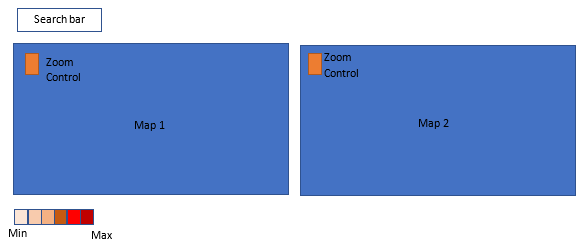
\includegraphics[width=.8\textwidth]{Pictures/FinalDesign}
	\caption{An illustration of the final design}
	\label{FinalDesignFig}
\end{figure}

The concept for a solution has been illustrated in figure \ref{FinalDesignFig}. The tool will use two maps with a shared view, so that both maps show the same area. Each map will show a different scenario, so that different population projections can be compared. Only the essential functionalities will be implemented in this prototype. The other useful functions would be excellent options for future work.


\subsection{Visualisation}
The sequential color scale chosen for the visualized rasters has been created by colorbrewer.org. It was decided to use six different colors on the maps. This is despite the fact that \citet{ColorBrewer} advise that more colors safely can be used, when similar colors are neighboring each other. The reason for this is that even though similar colors are neighboring each other within the individual map, the user still has to compare none-neighboring colors, since comparison is done between the two maps. The breakpoints between the different classes are determined as equal sized percentage steps of 20 \% of the current maximum value.  
%The mapped data is showing the population per square kilometre. It is therefore necessary that the area will not get distorted, so an equivalent projection is required. 

The projection EPSG:4326 was both used in Baumrock's original map and for the case data and will also be used for this project. The map will not be used to visualise data at a subcontinental scale, so the distortion from this projection, will not have serious consequences. The reason for this limit in scale is the time and diskspace required to create the tiles, which will be expanded upon in section \ref{TilesTime}.
